\subsection{Tests results for those who can't wait}

OpenICAMINUIT (ICA v. 1.4 x) was tested against several simulated datasets that were developped in 2004 to test ICA version 1.4 w \citep{kieTR05}. As ICA 1.4 w had estimated perfectly the parameters used to simulate the fishery datasets, we used them as a benchmarck for OpenICA.

OpenICAMINUIT is still under development: DO NOT USE THIS VERSION OF ICA FOR OTHER PURPOSES THAN TESTING !

\subsection{Detailed tests results}

These tests were performed on set of data available \htmladdnormallink{here}{./test/datasets}.

\subsubsection{Deterministic datasets, fitting surveys as absolute measurements of SSB}

This dataset was developed to test ICA version 1.4 w \citep{kieTR05}: it estimated its paramaters with a precision inferior to 0.01\%. 

The tests were performed using 10 sets of data that simulated a fishery occuring between 1972 and 2002 (31 years). The total number of TSB, SSB and recruitment values estimated by OpenICAMINUIT and compared in the figures below were 310. To create the simulated dataset, recruitment values were resampled from the 2002 WGMHSA official ICA run which was a set of 29 recruitment values.

This set of data was used to check OpenICAMINUIT (ICA version 1.4x) estimates of Spawning Stock Biomass (SSB), Total Stock Biomass (TSB), recruitment and fishing mortality. The results are shown below.

\begin{figure}
	\begin{center}
	\fbox{ 
	  \epsfig{width=5in,file=/home/mkienzle/CSIRO/cmar_projects/Fortran/ICA/OpenICAMINUIT/Tests/Results/Absolute-NoVariability-NoSSBbias-NoCatchBias-SSBsurveyNVNVNV/comparison-ssb.ps}
	}
	\end{center}
	\caption{Comparison of the Spawning Stock Biomass estimates from Open ICA (version 1.4x) against parameters used to simulate data. NB: the line correspond to y=x.}
\end{figure}

 \begin{figure}
  	\begin{center}
  	\fbox{ 
  	  \epsfig{width=5in,file=/home/mkienzle/CSIRO/cmar_projects/Fortran/ICA/OpenICAMINUIT/Tests/Results/Absolute-NoVariability-NoSSBbias-NoCatchBias-SSBsurveyNVNVNV/comparison-tsb.ps}
  	}
  	\end{center}
  	\caption{Comparison of the Total Stock Biomass estimates from Open ICA (version 1.4x) against parameters used to simulate data. NB: the line correspond to y=x.}
  \end{figure}

  \begin{figure}
  	\begin{center}
  	\fbox{ 
  	  \epsfig{width=5in,file=/home/mkienzle/CSIRO/cmar_projects/Fortran/ICA/OpenICAMINUIT/Tests/Results/Absolute-NoVariability-NoSSBbias-NoCatchBias-SSBsurveyNVNVNV/comparison-recruitment.ps}
  	}
  	\end{center}
  	\caption{Comparison of the recruitment estimates from Open ICA (version 1.4x) against parameters used to simulate data. NB: the line correspond to y=x.}
  \end{figure}

  %% \begin{figure}
  %% 	\begin{center}
  %% 	\fbox{ 
  %% 	  \epsfig{width=5in,file=../../Tests/Results/Absolute-NoVariability-NoSSBbias-NoCatchBias-SSBsurveyNVNVNV/comparison-Fbar.ps}
  %% 	}
  %% 	\end{center}
  %% 	\caption{Comparison of the $\bar{F}$ estimates from ICA version 1.4w against 1.4x. NB: the line correspond to y=x.}
  %% \end{figure}

\subsubsection{Deterministic datasets, fitting surveys as relative measurements of SSB}

This dataset was developed to test ICA version 1.4 w \citep{kieTR05}: it estimated its paramaters with a precision inferior to 0.01\%. 

The tests were performed using 10 sets of data that simulated a fishery occuring between 1972 and 2002 (31 years). The total number of TSB, SSB and recruitment values estimated by OpenICAMINUIT and compared in the figures below were 310. To create the simulated dataset, recruitment values were resampled from the 2002 WGMHSA official ICA run which was a set of 29 recruitment values.

This set of data was used to check OpenICAMINUIT (ICA version 1.4x) estimates of Spawning Stock Biomass (SSB), Total Stock Biomass (TSB), recruitment and fishing mortality. The results are shown below.

\begin{figure}
	\begin{center}
	\fbox{ 
	  \epsfig{width=5in,file=/home/mkienzle/CSIRO/cmar_projects/Fortran/ICA/OpenICAMINUIT/Tests/Results/Relative-NoVariability-NoSSBbias-NoCatchBias-SSBsurveyNVNVNV/comparison-ssb.ps}
	}
	\end{center}
	\caption{Comparison of the Spawning Stock Biomass estimates from Open ICA (version 1.4x) against parameters used to simulate data. NB: the line correspond to y=x.}
\end{figure}

 \begin{figure}
  	\begin{center}
  	\fbox{ 
  	  \epsfig{width=5in,file=/home/mkienzle/CSIRO/cmar_projects/Fortran/ICA/OpenICAMINUIT/Tests/Results/Relative-NoVariability-NoSSBbias-NoCatchBias-SSBsurveyNVNVNV/comparison-tsb.ps}
  	}
  	\end{center}
  	\caption{Comparison of the Total Stock Biomass estimates from Open ICA (version 1.4x) against parameters used to simulate data. NB: the line correspond to y=x.}
  \end{figure}

  \begin{figure}
  	\begin{center}
  	\fbox{ 
  	  \epsfig{width=5in,file=/home/mkienzle/CSIRO/cmar_projects/Fortran/ICA/OpenICAMINUIT/Tests/Results/Relative-NoVariability-NoSSBbias-NoCatchBias-SSBsurveyNVNVNV/comparison-recruitment.ps}
  	}
  	\end{center}
  	\caption{Comparison of the recruitment estimates from Open ICA (version 1.4x) against parameters used to simulate data. NB: the line correspond to y=x.}
  \end{figure}

  %% \begin{figure}
  %% 	\begin{center}
  %% 	\fbox{ 
  %% 	  \epsfig{width=5in,file=../../Tests/Results/Relative-NoVariability-NoSSBbias-NoCatchBias-SSBsurveyNVNVNV/comparison-Fbar.ps}
  %% 	}
  %% 	\end{center}
  %% 	\caption{Comparison of the $\bar{F}$ estimates from ICA version 1.4w against 1.4x. NB: the line correspond to y=x.}
  %% \end{figure}

